% Source reference: :contentReference[oaicite:0]{index=0}
\part{Graph Theory}
\section{Handout 09: Graph Theory (3): Graph Coloring, Planar Graphs}

\subsection{Overview}

This handout studies two major graph-theoretic themes:
\begin{itemize}[leftmargin=*]
    \item \emph{vertex coloring}: assigning colors to vertices so that adjacent vertices receive different colors;
    \item \emph{planarity}: drawing graphs in the plane without edge crossings.
\end{itemize}

The key topics are:
\begin{itemize}[leftmargin=*]
    \item \(k\)-vertex-colorings and chromatic number \(\chi(G)\);
    \item bipartite graphs as exactly the graphs that are \(2\)-colorable;
    \item complete bipartite graphs \(K_{m,n}\);
    \item planar representations and regions;
    \item Euler's formula for connected planar graphs;
    \item edge-count tests for non-planarity;
    \item non-planarity of \(K_5\) and \(K_{3,3}\);
    \item map coloring and the Four-Color Theorem.
\end{itemize}

\begin{examtip}[title={Main diagnostic for Handout 09}]
When facing a problem from this handout, first decide whether it is asking about:
\[
\begin{aligned}
&\text{coloring vertices}, && \text{splitting vertices into two parts},\\
&\text{drawing without crossings}, && \text{proving non-planarity}.
\end{aligned}
\]
These require different tools.
\end{examtip}

%==================================================
\subsection{Vertex Coloring}
%==================================================

\begin{definition}{\(k\)-vertex-coloring}{vertex-coloring}
Let \(G=(V,E)\) be a graph. A \emph{\(k\)-vertex-coloring} of \(G\) is a function
\[
f:V\to \{1,2,\dots,k\}
\]
such that whenever \(u\) and \(v\) are adjacent,
\[
\{u,v\}\in E
\quad\Longrightarrow\quad
f(u)\neq f(v).
\]
\end{definition}

Thus adjacent vertices must receive different colors. Non-adjacent vertices may receive the same color.

\begin{definition}{\(k\)-colorable graph and chromatic number}{chromatic-number}
A graph \(G\) is \emph{\(k\)-colorable} if it has a \(k\)-vertex-coloring.

The \emph{chromatic number} of \(G\), denoted \(\chi(G)\), is the smallest integer \(k\) such that \(G\) is \(k\)-colorable.
\end{definition}

\begin{keyformula}[title={Meaning of chromatic number}]
\[
\chi(G)=\min\{k:\ G\text{ has a valid }k\text{-vertex-coloring}\}.
\]
\end{keyformula}

% Example of a proper 4-coloring of a small graph.
\begin{center}
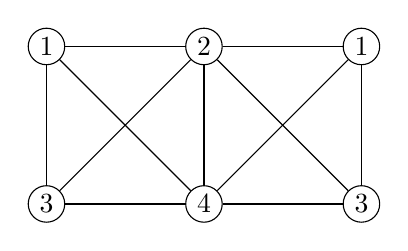
\begin{tikzpicture}[scale=1.0]
    \node[circle,draw,inner sep=1.8pt] (a) at (0,1) {$1$};
    \node[circle,draw,inner sep=1.8pt] (b) at (2,1) {$2$};
    \node[circle,draw,inner sep=1.8pt] (c) at (4,1) {$1$};
    \node[circle,draw,inner sep=1.8pt] (d) at (0,-1) {$3$};
    \node[circle,draw,inner sep=1.8pt] (e) at (2,-1) {$4$};
    \node[circle,draw,inner sep=1.8pt] (f) at (4,-1) {$3$};

    \draw (a)--(b)--(c);
    \draw (d)--(e)--(f);
    \draw (a)--(d);
    \draw (b)--(e);
    \draw (c)--(f);
    \draw (a)--(e);
    \draw (b)--(d);
    \draw (b)--(f);
    \draw (c)--(e);
\end{tikzpicture}
\end{center}

\begin{examplebox}[title={Basic chromatic numbers}]
For complete graphs,
\[
\chi(K_n)=n,
\]
because every pair of vertices is adjacent.

For cycle graphs,
\[
\chi(C_n)=
\begin{cases}
2, & n\text{ even},\\
3, & n\text{ odd}.
\end{cases}
\]
Also,
\[
\chi(G)=1
\]
if and only if \(G\) has no edges.
\end{examplebox}

\begin{proof}
For \(K_n\), every pair of vertices is adjacent, so all \(n\) vertices must receive distinct colors. Hence \(\chi(K_n)=n\).

For \(C_n\), if \(n\) is even, alternate two colors around the cycle. If \(n\) is odd, two colors cannot close consistently around the cycle, but three colors suffice. Thus the stated formula holds.
\end{proof}

\begin{commonmistake}[title={Color labels are arbitrary}]
A coloring is not about the names of colors. If two colorings differ only by renaming colors, they represent the same coloring structure. What matters is whether adjacent vertices have different colors.
\end{commonmistake}

%==================================================
\subsection{Bipartite Graphs}
%==================================================

\begin{definition}{Bipartite graph}{bipartite-graph}
A simple graph \(G=(V,E)\) is \emph{bipartite} if its vertex set can be partitioned as
\[
V=V_L\sqcup V_R
\]
such that every edge of \(G\) has one endpoint in \(V_L\) and one endpoint in \(V_R\). The pair
\[
(V_L,V_R)
\]
is called a \emph{bipartition} of \(V\).
\end{definition}

Equivalently, a bipartite graph has no edges inside \(V_L\) and no edges inside \(V_R\).

% Bipartite graph layout with left and right vertex classes.
\begin{center}
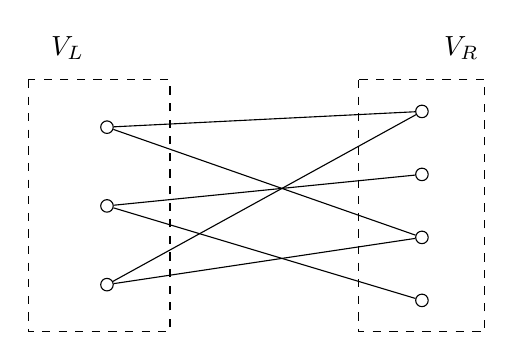
\begin{tikzpicture}[scale=1.0]
    \node at (-1.5,2.0) {$V_L$};
    \node at (3.5,2.0) {$V_R$};

    \node[circle,draw,inner sep=1.6pt] (a) at (-1,1) {};
    \node[circle,draw,inner sep=1.6pt] (b) at (-1,0) {};
    \node[circle,draw,inner sep=1.6pt] (c) at (-1,-1) {};

    \node[circle,draw,inner sep=1.6pt] (d) at (3,1.2) {};
    \node[circle,draw,inner sep=1.6pt] (e) at (3,0.4) {};
    \node[circle,draw,inner sep=1.6pt] (f) at (3,-0.4) {};
    \node[circle,draw,inner sep=1.6pt] (g) at (3,-1.2) {};

    \draw (a)--(d);
    \draw (a)--(f);
    \draw (b)--(e);
    \draw (b)--(g);
    \draw (c)--(d);
    \draw (c)--(f);

    \draw[dashed] (-2,1.6) rectangle (-0.2,-1.6);
    \draw[dashed] (2.2,1.6) rectangle (3.8,-1.6);
\end{tikzpicture}
\end{center}

\begin{theorem}{Bipartite graphs and \(2\)-colorability}{bipartite-two-colorable}
A graph \(G\) is bipartite if and only if
\[
\chi(G)\le 2.
\]
\end{theorem}

\begin{proof}
Suppose \(G\) is bipartite with bipartition
\[
V=V_L\sqcup V_R.
\]
Color all vertices in \(V_L\) with color \(1\), and all vertices in \(V_R\) with color \(2\). Since every edge goes between the two parts, this is a valid \(2\)-coloring. Hence \(\chi(G)\le 2\).

Conversely, suppose \(\chi(G)\le 2\). If \(G\) has a \(1\)-coloring, then \(G\) has no edges and is bipartite. If \(G\) has a \(2\)-coloring, let \(V_L\) be the set of vertices of color \(1\), and \(V_R\) the set of vertices of color \(2\). Adjacent vertices have different colors, so every edge goes between \(V_L\) and \(V_R\). Hence \(G\) is bipartite.
\end{proof}

\begin{theorem}{Odd-cycle characterization of bipartite graphs}{bipartite-odd-cycle}
A graph is bipartite if and only if it contains no odd cycle as a subgraph.
\end{theorem}

\begin{proof}
If \(G\) is bipartite, every cycle must alternate between the two parts \(V_L\) and \(V_R\). Returning to the starting vertex is possible only after an even number of steps. Hence every cycle in a bipartite graph has even length.

Conversely, if \(G\) has no odd cycle, one may color each connected component by choosing a starting vertex, coloring vertices at even distance from it with one color and vertices at odd distance from it with another. The absence of odd cycles ensures this is well-defined and produces a valid bipartition.
\end{proof}

\begin{examplebox}[title={Tutorial 9, Question 3}]
For \(K_n\), the graph is bipartite exactly when
\[
n=1\quad\text{or}\quad n=2.
\]
Indeed, \(K_n\) contains a triangle whenever \(n\ge 3\), and a triangle is an odd cycle.

For \(C_n\),
\[
C_n\text{ is bipartite}
\quad\Longleftrightarrow\quad
n\text{ is even}.
\]
This follows directly from the odd-cycle characterization.
\end{examplebox}

\begin{examtip}[title={Fast tests for bipartiteness}]
To prove a graph is bipartite, exhibit a bipartition or a \(2\)-coloring.

To prove it is not bipartite, find an odd cycle.
\end{examtip}

%==================================================
\subsection{Complete Bipartite Graphs}
%==================================================

\begin{definition}{Complete bipartite graph}{complete-bipartite}
The \emph{complete bipartite graph} \(K_{m,n}\) has vertex set
\[
V=V_1\sqcup V_2,
\qquad |V_1|=m,\quad |V_2|=n,
\]
with no edges inside \(V_1\) or inside \(V_2\), and with every vertex of \(V_1\) adjacent to every vertex of \(V_2\).
\end{definition}

\begin{keyformula}[title={Basic data for \(K_{m,n}\)}]
\[
|V(K_{m,n})|=m+n,
\qquad
|E(K_{m,n})|=mn.
\]
Each vertex in the \(m\)-part has degree \(n\), and each vertex in the \(n\)-part has degree \(m\).
\end{keyformula}

% Complete bipartite graph K_{3,3}.
\begin{center}
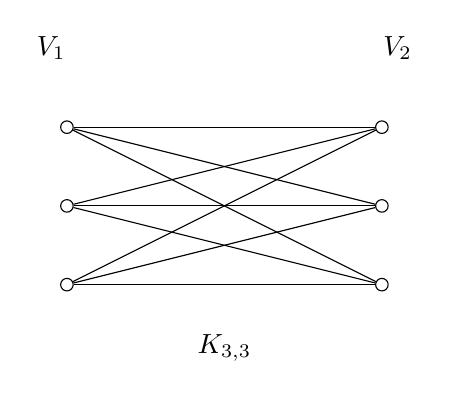
\begin{tikzpicture}[scale=1.0]
    \node at (-1.2,2.0) {$V_1$};
    \node at (3.2,2.0) {$V_2$};

    \foreach \i/\y in {1/1,2/0,3/-1}{
        \node[circle,draw,inner sep=1.6pt] (L\i) at (-1,\y) {};
    }
    \foreach \i/\y in {1/1,2/0,3/-1}{
        \node[circle,draw,inner sep=1.6pt] (R\i) at (3,\y) {};
    }

    \foreach \i in {1,2,3}{
        \foreach \j in {1,2,3}{
            \draw (L\i)--(R\j);
        }
    }

    \node at (1,-1.8) {$K_{3,3}$};
\end{tikzpicture}
\end{center}

\begin{examplebox}[title={Tutorial 9, Question 4}]
The degree sequence of \(K_{2,3}\) is
\[
3,3,2,2,2.
\]
For \(K_{m,n}\), the \(m\) vertices on one side each have degree \(n\), while the \(n\) vertices on the other side each have degree \(m\). Thus, if \(m\le n\), the degree sequence is
\[
\underbrace{n,n,\dots,n}_{m\text{ terms}},
\underbrace{m,m,\dots,m}_{n\text{ terms}}.
\]
\end{examplebox}

\begin{extension}[title={Adjacency-matrix viewpoint}]
If the vertices are ordered by the two parts of \(K_{m,n}\), then its adjacency matrix has block form
\[
\begin{pmatrix}
0 & J_{m\times n}\\
J_{n\times m} & 0
\end{pmatrix},
\]
where \(J\) is an all-ones matrix. Row sums immediately give the degree sequence.
\end{extension}

%==================================================
\subsection{Planar Graphs}
%==================================================

\begin{definition}{Planar graph and planar representation}{planar-graph}
A graph is \emph{planar} if it can be drawn in the plane so that no two edges cross except possibly at common endpoints.

A drawing with no such crossings is called a \emph{planar representation} of the graph.
\end{definition}

Planarity is a property of the abstract graph, not of one particular drawing. A graph may look non-planar in one drawing but still be planar if a different crossing-free drawing exists.

\begin{examplebox}[title={\(K_4\) is planar}]
The graph \(K_4\) may be drawn with crossings if all four vertices are placed on a square and both diagonals are drawn. However, it has a planar representation by placing one vertex inside a triangle and joining it to the three triangle vertices. Hence \(K_4\) is planar.
\end{examplebox}

% Planar drawing of K4 with one vertex inside a triangle.
\begin{center}
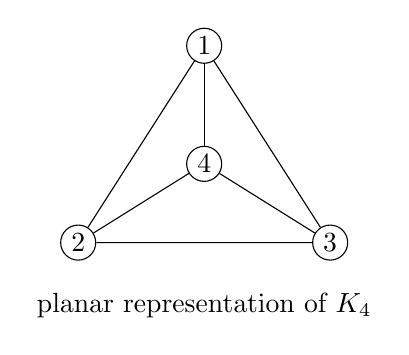
\begin{tikzpicture}[scale=1.0]
    \node[circle,draw,inner sep=1.6pt] (a) at (0,1.5) {$1$};
    \node[circle,draw,inner sep=1.6pt] (b) at (-1.6,-1) {$2$};
    \node[circle,draw,inner sep=1.6pt] (c) at (1.6,-1) {$3$};
    \node[circle,draw,inner sep=1.6pt] (d) at (0,0) {$4$};

    \draw (a)--(b)--(c)--(a);
    \draw (d)--(a);
    \draw (d)--(b);
    \draw (d)--(c);

    \node at (0,-1.8) {planar representation of \(K_4\)};
\end{tikzpicture}
\end{center}

\begin{commonmistake}[title={A non-planar-looking drawing is not a proof}]
To prove that a graph is non-planar, it is not enough to show one drawing with crossings. One must prove that \emph{no} crossing-free drawing exists.
\end{commonmistake}

%==================================================
\subsection{Regions and Euler's Formula}
%==================================================

\begin{definition}{Region / face}{region-face}
A planar representation of a graph divides the plane into \emph{regions}, also called \emph{faces}. One of these is the unbounded outside region, called the \emph{infinite region}.
\end{definition}

\begin{definition}{Degree of a region}{region-degree}
The \emph{degree} of a region \(R\), denoted \(\deg(R)\), is the number of edge-boundary occurrences around \(R\). If an edge appears twice on the boundary of a region, it contributes twice to \(\deg(R)\).
\end{definition}

% Planar graph with three regions labelled.
\begin{center}
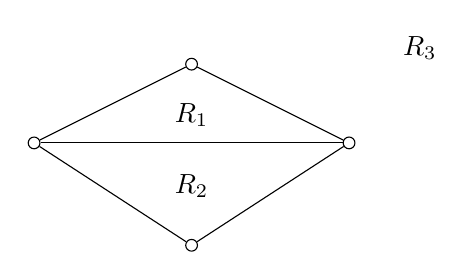
\begin{tikzpicture}[scale=1.0]
    \node[circle,draw,inner sep=1.5pt] (a) at (0,0) {};
    \node[circle,draw,inner sep=1.5pt] (b) at (2,1) {};
    \node[circle,draw,inner sep=1.5pt] (c) at (4,0) {};
    \node[circle,draw,inner sep=1.5pt] (d) at (2,-1.3) {};

    \draw (a)--(b)--(c)--(d)--(a);
    \draw (a)--(c);

    \node at (2,0.35) {\(R_1\)};
    \node at (2,-0.55) {\(R_2\)};
    \node at (4.9,1.2) {\(R_3\)};
\end{tikzpicture}
\end{center}

\begin{theorem}{Euler's Formula}{euler-formula}
Let \(G\) be a connected planar simple graph with
\[
n=|V|,\qquad m=|E|,
\]
and let \(r\) be the number of regions in a planar representation of \(G\). Then
\[
n-m+r=2.
\]
Equivalently,
\[
r=m-n+2.
\]
\end{theorem}

\begin{keyformula}[title={Euler's Formula}]
\[
n-m+r=2
\qquad
\text{for connected planar simple graphs.}
\]
\end{keyformula}

\begin{theorem}{Sum of the degrees of regions}{region-degree-sum}
In a planar representation of a planar graph,
\[
\sum_R \deg(R)=2m,
\]
where the sum is over all regions.
\end{theorem}

\begin{proof}
Every edge borders regions on its two sides. If the same region lies on both sides of an edge, that edge is counted twice in that region's boundary. Hence every edge contributes exactly \(2\) to the total sum of region degrees, so
\[
\sum_R\deg(R)=2m.
\]
\end{proof}

\begin{extension}[title={Dual handshaking idea}]
The identity
\[
\sum_R\deg(R)=2m
\]
is the face-version of the Handshaking Lemma. The usual Handshaking Lemma sums degrees over vertices; this one sums boundary degrees over regions.
\end{extension}

%==================================================
\subsection{Edge Bounds for Planar Graphs}
%==================================================

\begin{theorem}{Planar edge bound}{planar-edge-bound}
If \(G\) is a connected planar simple graph with \(n\ge 3\) vertices and \(m\) edges, then
\[
m\le 3n-6.
\]
\end{theorem}

\begin{proof}
Every region has degree at least \(3\), so
\[
2m=\sum_R\deg(R)\ge 3r.
\]
Hence
\[
r\le \frac{2m}{3}.
\]
Using Euler's formula,
\[
2=n-m+r\le n-m+\frac{2m}{3}=n-\frac{m}{3}.
\]
Thus
\[
m\le 3n-6.
\]
\end{proof}

\begin{theorem}{Triangle-free planar edge bound}{triangle-free-planar-bound}
If \(G\) is a connected simple planar graph with \(n\ge 3\) vertices, \(m\) edges, and no cycles of length \(3\), then
\[
m\le 2n-4.
\]
\end{theorem}

\begin{proof}
Since \(G\) has no \(3\)-cycles, every region has boundary degree at least \(4\). Thus
\[
2m=\sum_R\deg(R)\ge 4r,
\]
so
\[
r\le \frac{m}{2}.
\]
Euler's formula gives
\[
2=n-m+r\le n-m+\frac{m}{2}=n-\frac{m}{2}.
\]
Therefore
\[
m\le 2n-4.
\]
\end{proof}

\begin{keyformula}[title={Fast planar non-planarity tests}]
For simple planar graphs:
\[
m\le 3n-6
\qquad (n\ge 3).
\]
If there are no triangles:
\[
m\le 2n-4.
\]
Violating either relevant bound proves non-planarity.
\end{keyformula}

\begin{commonmistake}[title={These inequalities are one-way tests}]
If a graph violates the planar edge bound, it is non-planar. But satisfying the bound does \emph{not} guarantee planarity.
\end{commonmistake}

%==================================================
\subsection{Non-Planarity of \(K_5\) and \(K_{3,3}\)}
%==================================================

\begin{examplebox}[title={Non-planarity of \(K_5\)}]
The complete graph \(K_5\) has
\[
n=5,\qquad m=\binom{5}{2}=10.
\]
If \(K_5\) were planar, then the planar edge bound would give
\[
m\le 3n-6=3(5)-6=9.
\]
But
\[
10\le 9
\]
is false. Hence
\[
\boxed{K_5\text{ is not planar}.}
\]
\end{examplebox}

\begin{examplebox}[title={Non-planarity of \(K_{3,3}\)}]
The complete bipartite graph \(K_{3,3}\) has
\[
n=6,\qquad m=9.
\]
It has no triangles because it is bipartite. If it were planar, the triangle-free planar bound would give
\[
m\le 2n-4=2(6)-4=8.
\]
But
\[
9\le 8
\]
is false. Therefore
\[
\boxed{K_{3,3}\text{ is not planar}.}
\]
\end{examplebox}

\begin{examplebox}[title={Tutorial 9, Question 5}]
Removing one edge from \(K_{3,3}\) gives a graph with
\[
n=6,\qquad m=8.
\]
This no longer violates the triangle-free planar bound
\[
m\le 2n-4=8.
\]
Indeed, \(K_{3,3}\) with one edge removed has a planar drawing.

Similarly, removing one edge from \(K_5\) gives
\[
n=5,\qquad m=9,
\]
which no longer violates
\[
m\le 3n-6=9.
\]
Indeed, \(K_5\) with one edge removed is planar.
\end{examplebox}

\begin{examtip}[title={Choosing the right edge bound}]
Use
\[
m\le 3n-6
\]
for general simple planar graphs.

Use
\[
m\le 2n-4
\]
when the graph has no triangles, especially for bipartite graphs such as \(K_{3,3}\).
\end{examtip}

%==================================================
\subsection{Disconnected Planar Graphs}
%==================================================

The edge-count corollaries are often applied componentwise or by adding edges between components.

\begin{theorem}{Planar edge bounds for disconnected simple graphs}{disconnected-planar-bounds}
Let \(G\) be a simple planar graph with \(n\ge 3\) vertices and \(m\) edges. Then
\[
m\le 3n-6.
\]
If \(G\) has no cycles of length \(3\), then
\[
m\le 2n-4.
\]
\end{theorem}

\begin{proof}
If \(G\) is disconnected, add edges between connected components in a planar drawing until the graph becomes connected. This does not destroy planarity. The resulting connected planar graph has at least \(m\) edges and the same \(n\) vertices. Applying the connected case gives the same upper bound for the original graph.
\end{proof}

\begin{extension}[title={Why adding edges can help prove an upper bound}]
Adding edges to connect components can only increase the edge count. If the larger connected planar graph must satisfy an upper bound, then the original disconnected graph also satisfies it.
\end{extension}

%==================================================
\subsection{Homeomorphic Graphs and Kuratowski's Theorem}
%==================================================

\begin{definition}{Elementary subdivision}{elementary-subdivision}
An \emph{elementary subdivision} of an edge \(\{u,v\}\) removes the edge \(\{u,v\}\), adds a new vertex \(w\), and inserts the two edges
\[
\{u,w\},\qquad \{w,v\}.
\]
\end{definition}

\begin{definition}{Homeomorphic graphs}{homeomorphic-graphs}
Two graphs are \emph{homeomorphic} if they can be obtained from the same graph by a sequence of elementary subdivisions.
\end{definition}

% Elementary subdivision of an edge.
\begin{center}
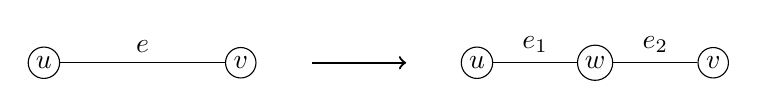
\begin{tikzpicture}[scale=1.0]
    \node[circle,draw,inner sep=1.5pt] (u1) at (0,0) {\(u\)};
    \node[circle,draw,inner sep=1.5pt] (v1) at (2.5,0) {\(v\)};
    \draw (u1)--node[above]{\(e\)}(v1);

    \draw[->,thick] (3.4,0)--(4.6,0);

    \node[circle,draw,inner sep=1.5pt] (u2) at (5.5,0) {\(u\)};
    \node[circle,draw,inner sep=1.5pt] (w) at (7.0,0) {\(w\)};
    \node[circle,draw,inner sep=1.5pt] (v2) at (8.5,0) {\(v\)};
    \draw (u2)--node[above]{\(e_1\)}(w)--node[above]{\(e_2\)}(v2);
\end{tikzpicture}
\end{center}

\begin{theorem}{Kuratowski's Theorem}{kuratowski}
A graph is non-planar if and only if it contains a subgraph homeomorphic to either
\[
K_5
\qquad\text{or}\qquad
K_{3,3}.
\]
\end{theorem}

\begin{extension}[title={How to interpret Kuratowski's Theorem}]
Kuratowski's Theorem says that \(K_5\) and \(K_{3,3}\) are the two fundamental obstructions to planarity, up to subdivision. In practice, the theorem is useful for recognizing hidden non-planar structure inside a larger graph.
\end{extension}

%==================================================
\subsection{Map Coloring and the Four-Color Theorem}
%==================================================

Map coloring can be converted into graph coloring. Represent each region of a map by a vertex. Join two vertices by an edge if the corresponding regions share a boundary segment.

\begin{definition}{Map adjacency graph}{map-adjacency-graph}
Given a map divided into regions, its \emph{adjacency graph} has:
\begin{itemize}[leftmargin=*]
    \item one vertex for each region;
    \item an edge between two vertices if the corresponding regions share a common boundary segment.
\end{itemize}
Touching at only a corner does not count as adjacency.
\end{definition}

\begin{theorem}{Four-Color Theorem}{four-color-theorem}
Every simple planar graph is \(4\)-colorable.
\end{theorem}

\begin{keyformula}[title={Four-Color Theorem}]
\[
G\text{ simple and planar}
\quad\Longrightarrow\quad
\chi(G)\le 4.
\]
\end{keyformula}

\begin{examplebox}[title={Map coloring as graph coloring}]
To color a map, construct the region-adjacency graph. A valid coloring of the map is then exactly a valid vertex-coloring of this graph.
\end{examplebox}

\begin{commonmistake}[title={Four colors is an upper bound, not always the exact value}]
The Four-Color Theorem says
\[
\chi(G)\le 4
\]
for every simple planar graph \(G\). It does not say that every planar graph has chromatic number exactly \(4\). Many planar graphs are \(1\)-, \(2\)-, or \(3\)-colorable.
\end{commonmistake}

\begin{examplebox}[title={Tutorial 9, Question 6}]
A planar graph can have chromatic number \(4\). The standard example is
\[
K_4.
\]
It is planar, and since every pair of vertices is adjacent,
\[
\chi(K_4)=4.
\]
Thus \(K_4\) shows that the Four-Color Theorem is sharp.
\end{examplebox}

%==================================================
\subsection{Special Techniques}
%==================================================

\subsubsection*{1. Prove colorability by constructing a coloring}
To show \(\chi(G)\le k\), explicitly give a \(k\)-coloring or describe a coloring algorithm.

\subsubsection*{2. Prove lower bounds by finding cliques or odd cycles}
If \(G\) contains a copy of \(K_t\), then
\[
\chi(G)\ge t.
\]
If \(G\) contains an odd cycle, then
\[
\chi(G)\ge 3.
\]

\subsubsection*{3. Prove bipartiteness using a bipartition}
For a positive result, explicitly write
\[
V=V_L\sqcup V_R
\]
and check that every edge crosses between the parts.

\subsubsection*{4. Disprove bipartiteness using an odd cycle}
A single odd cycle is enough to prove that a graph is not bipartite.

\subsubsection*{5. Prove planarity by drawing}
To prove a graph is planar, it is enough to provide one crossing-free planar representation.

\subsubsection*{6. Prove non-planarity using edge bounds}
For simple graphs, first test:
\[
m\le 3n-6.
\]
For triangle-free graphs, especially bipartite graphs, test:
\[
m\le 2n-4.
\]

\subsubsection*{7. Use Kuratowski's Theorem for hidden obstructions}
If the edge-count inequalities do not prove non-planarity, search for a subdivision of \(K_5\) or \(K_{3,3}\).

\begin{extension}[title={Fast decision tree for Handout 09}]
\[
\begin{array}{c|c}
\text{Question type} & \text{Fast first move} \\ \hline
\text{Is the graph bipartite?} & \text{try a 2-coloring or find an odd cycle} \\
\text{Find }\chi(G) & \text{give upper coloring and lower obstruction} \\
\text{Is the graph planar?} & \text{try drawing it without crossings} \\
\text{Prove non-planarity} & \text{test edge bounds, then search for }K_5/K_{3,3}
\end{array}
\]
A complete solution often needs both an upper bound and a lower bound.
\end{extension}

%==================================================
\subsection{Summary Table}
%==================================================

\begin{center}
\small
\begin{tabular}{@{}p{0.28\textwidth}p{0.30\textwidth}p{0.31\textwidth}@{}}
\toprule
\textbf{Concept} & \textbf{Definition / formula} & \textbf{Exam use} \\
\midrule
\(k\)-coloring & \(f:V\to\{1,\dots,k\}\), adjacent vertices different & prove colorability \\
Chromatic number & \(\chi(G)=\min k\) for valid \(k\)-coloring & exact color requirement \\
Bipartite graph & \(V=V_L\sqcup V_R\), all edges cross parts & equivalent to \(\chi(G)\le 2\) \\
Odd-cycle criterion & bipartite \(\Longleftrightarrow\) no odd cycle & fast non-bipartite test \\
Complete bipartite graph & \(K_{m,n}\), all cross edges present & \(|E|=mn\) \\
Planar graph & drawable without crossings & one drawing proves planarity \\
Euler's formula & \(n-m+r=2\) & connected planar graphs \\
Region degree sum & \(\sum_R\deg(R)=2m\) & derive edge bounds \\
Planar edge bound & \(m\le 3n-6\) & fast non-planarity test \\
Triangle-free bound & \(m\le 2n-4\) & useful for bipartite graphs \\
Kuratowski obstruction & contains subdivision of \(K_5\) or \(K_{3,3}\) & deeper non-planarity test \\
Four-Color Theorem & planar simple graph \(\Rightarrow \chi(G)\le 4\) & map coloring upper bound \\
\bottomrule
\end{tabular}
\end{center}

\begin{examtip}[title={Final checklist for Handout 09}]
Before finalizing a solution, check:
\begin{enumerate}[leftmargin=*]
    \item If proving colorability, did you give a valid coloring?
    \item If proving a chromatic number exactly, did you prove both upper and lower bounds?
    \item If proving bipartiteness, did you give a bipartition or use the odd-cycle criterion?
    \item If proving planarity, did you provide a crossing-free drawing?
    \item If proving non-planarity, did you use a valid obstruction rather than relying on a bad drawing?
\end{enumerate}
\end{examtip}

\begin{commonmistake}[title={Final warning for Handout 09}]
A drawing with crossing edges proves nothing by itself. Planarity is about whether \emph{some} crossing-free drawing exists. Conversely, coloring a graph with too many colors gives only a weak upper bound; to find \(\chi(G)\), one must also prove that fewer colors are impossible.
\end{commonmistake}
